\documentclass{scrartcl}
\usepackage[margin=3cm]{geometry}
\usepackage{amsmath}
\usepackage{amssymb}
\usepackage{amsthm}
\usepackage{blindtext}
\usepackage{datetime}
\usepackage{fontspec}
\usepackage{float}
\usepackage{graphicx}
\usepackage{kotex}
\usepackage[lighttt]{lmodern}
\usepackage{listings}
\usepackage{mathrsfs}
\usepackage{mathtools}
\usepackage{pgf,tikz,pgfplots}
\usepackage{pdfpages}

\pgfplotsset{compat=1.15}
\usetikzlibrary{arrows}
\newtheorem{theorem}{Theorem}

\lstset{
  numbers=none, frame=single, showspaces=false,
  showstringspaces=false, showtabs=false, breaklines=true, showlines=true,
  breakatwhitespace=true, basicstyle=\ttfamily, keywordstyle=\bfseries, basewidth=0.5em
}

\setmainhangulfont{Noto Serif CJK KR}[
  UprightFont=* Light, BoldFont=* Bold,
  Script=Hangul, Language=Korean, AutoFakeSlant,
]
\setsanshangulfont{Noto Sans CJK KR}[
  UprightFont=* DemiLight, BoldFont=* Medium,
  Script=Hangul, Language=Korean
]
\setmathhangulfont{Noto Sans CJK KR}[
  SizeFeatures={
    {Size=-6,  Font=* Medium},
    {Size=6-9, Font=*},
    {Size=9-,  Font=* DemiLight},
  },
  Script=Hangul, Language=Korean
]
\title{CSED311: Lab 2 (due Mar. 26)}
\author{김태연(20220140), 손량(20220323)}
\date{Last compiled on: \today, \currenttime}

\newcommand{\un}[1]{\ensuremath{\ \mathrm{#1}}}

\begin{document}
\maketitle

\section{Introduction}
RISC-V architecture를 바탕으로 구성된 Single cycle CPU가 작동하는 방식을 알아보고,
각 Instruction type에 따라 거치는 Datapath에 유의하며 CPU를 구성하는 각 module을
설계하고 연결하여 Single cycle CPU를 구현한다.

\section{Design}
이번에 구현한 RISC-V Single cycle CPU는 다음과 같은 주요 기능을 가진 Submodule로 나누었으며, 해당 값들을
생성하고 선택하기 위해 추가적으로 Adder와 Multiplexer를 구현하여 사용했다.

\subsection{Program Counter}
PC, 즉 프로그램 카운터는 주어진 Clock signal에 synchronous하게 신호에 따라 다음 PC address의 값을
현재 PC address에 대입한다. 출력된 PC address는 CPU 내에서 구현된 분기(\texttt{Bxx}),
점프(\texttt{JAL, JALR}) 등의 Instruction에 따라 (현재 PC + 4) 혹은 (임의의 Instruction address)로
값이 변화하게 된다.

\subsection{ALU}
Register에 저장되어있는 32bit integer 또는 Immediate generator을 통해 Instruction으로부터
생성된 32bit integer의 값을 읽어들인 후 정의된 연산의 ID에 따라 연산을 진행하며,
\texttt{always @(*)}를 사용하여 주어진 opcode에 해당하는 연산 결과를
CPU clock cycle과 asynchronous하게 \texttt{alu\_result}로 반환했다.
Textbook에 등장하는 \texttt{bcond}를 32bit 연산 결과의 LSB에 할당하여, 논리 연산의 경우
LSB 1bit만 사용하여 연산을 진행한다.

\subsection{Register file}
RV32I Architecture의 32bit Register 32개를 구현하였다. 레지스터의 값을 작성하는 것과 읽어오는 것은
서로 다르게 설계하였다.

\begin{itemize}
    \item Write -- \texttt{posedge clk} 에 따라 Clock signal에 synchronous하게
    레지스터를 수정한다.
    \item Read -- \texttt{always @} 문 밖에서 Clock signal에 asynchronous하게 
    레지스터의 값을 입력으로 들어온 \texttt{rs1} 및 \texttt{rs2}에 해당하는 레지스터를
    참조하여 출력하도록 연결을 구성했다.
\end{itemize}

\subsection{Data memory}
주어진 "Magic memory"는 32bit integer \texttt{MEM\_DEPTH = 16384}개로 구성되어있는 64KiB 메모리이다.
메모리에 값을 작성하는 것과 읽어오는 것은 레지스터와 마찬가지의 로직으로 설계하였다.

\begin{itemize}
    \item Write -- \texttt{posedge clk} 에 맞추어 \texttt{mem\_write} 신호가 주어진
    경우에만 synchronous하게 memory file을 수정한다.
    \item Read -- \texttt{always @} 문 밖에서 Clock signal과 asynchronous하게, \texttt{dmem\_addr}로
    주어진 메모리 주소에 \texttt{mem\_read} signal이 참인 경우에 \texttt{dout}에 assign하였다.
\end{itemize}

\subsection{Instruction memory}
Instruction memory는 32bit instruction \texttt{MEM\_DEPTH = 1024}개로 구성되어있는 4KiB 메모리이다.
Testbench (혹은 RV32I로 컴파일된 프로그램)의 각 bytecode를 읽어서 Lab 2에서 구현한 Single-cycle CPU가
실행할 수 있도록 저장한다. 32bit PC를 입력받아, 실제로 구현된 1024개 instruction을 저장할 수 있는 LSB를 제외한
하위 10bit에 해당하는 instruction index로 변환하여 해당 index의 instruction을 Clock 신호와
asynchronous하게 \texttt{dout} 으로 반환한다.

\subsection{Control unit}
어떤 Instruction type이던, LSB 7bit는 RV32I에서 opcode로 정의가 되어 있는 부분이다.
구현한 Control unit은 Clock에 asynchronous하게 Instruction의 LSB 7bit를 입력받아 해당 opcode에 대응되는
CPU control signal을 생성한다.

\subsection{Immediate generator}
RV32I instruction 중 immediate value를 가지는 instruction의 타입이 존재하며, 각 타입 별 Immediate value가
생성되는 부분들 또한 다르다. 본 Single cycle CPU에서는 32bit instruction을 입력받고, 주어진 ISA에서
구현해야할 type에 해당하는 I-type, SB-type, UJ-type, S-type의 Instruction의 Immediate generation에 해당하는
output으로 타입을 구분하여 Clock signal과 asynchronous하게 Immediate value를 출력하였다.

\subsection{Ecall unit}
프로그램의 종료를 판별하기 위한 Ecall의 구조를 정의하였으며, Clock signal과 asynchronous하게 수행된다.

\section{Implementation}

각 베릴로그 파일에 대한 설명은 다음과 같다.

\subsection{\texttt{cpu.v} -- 내부적인 Module을 연결하여 CPU 구성}
하위 모듈들을 모두 조합하여 Single cycle CPU의 전체적인 Schematic을 구성하였다. CPU의 전체적인 구성을 출력하기 위해
Vivado Xilinix를 통해 만들어진 Schematic을 첨부하였다.

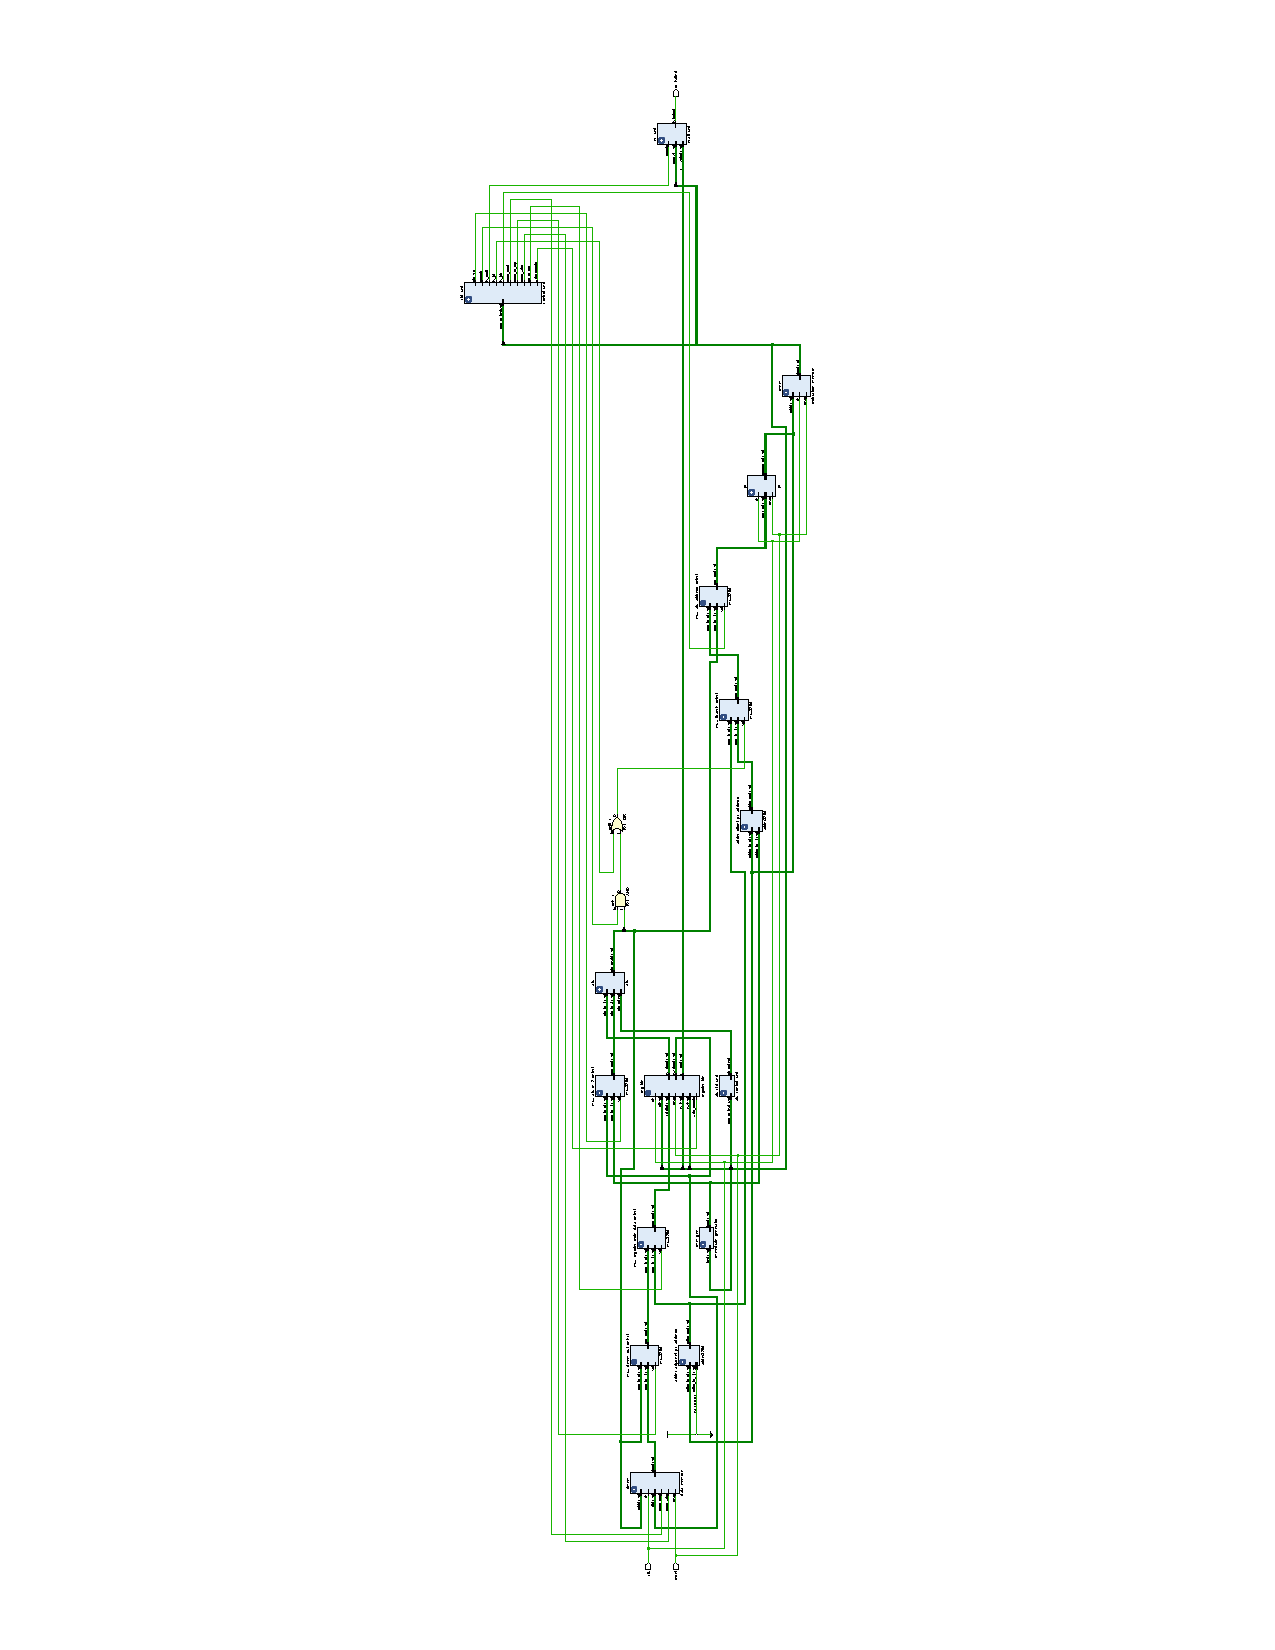
\includepdf[pages={1}, scale=1.05]{schematic.pdf}

\texttt{cpu.v}는 다음과 같은 submodule을 연결하여 구성했다.

\begin{itemize}
    \item \texttt{pc} -- Program counter를 구현하였다.
    \item \texttt{imem} -- Instruction memory를 구현하였다.
    \item \texttt{reg\_file} -- Register를 구현하였다.
    \item \texttt{ctrl\_unit} -- CPU Control unit을 구현하였다.
    \item \texttt{ec\_unit} -- \texttt{ecall} 을 처리하기 위한 unit을 구현하였다.
    \item \texttt{imm\_gen} -- 각 Instruction type으로부터 immediate value를 획득한다.
    \item \texttt{alu\_ctrl\_unit} -- Instruction으로부터 ALU의 opcode를 획득한다.
    \item \texttt{alu} -- ALU를 구현하였다.
    \item \texttt{dmem} -- Data memory를 구현하였다.
    \item \texttt{mux\_register\_write\_data\_select} -- Multiplexer로, (PC + 4) 혹은 Data memory의 출력을 선택하여 register file에 작성한다.
    \item \texttt{mux\_alu\_in\_2\_select} -- Multiplexer로, ALU에 들어갈 입력으로 immediate generator에서 생성한 immediate value 혹은 register의 값을 선택한다.
    \item \texttt{mux\_dmem\_out\_select} -- Multiplexer로, Write Back 단계에 사용할 출력으로 ALU의 출력 혹은 Data memory의 출력을 선택한다.
    \item \texttt{adder\_adjacent\_pc\_address} -- 인접한 다음 PC (PC + 4)를 계산하기 위해 존재하는 32bit adder이다. 두 번째 입력은 4로 고정되어있다.
    \item \texttt{adder\_offset\_pc\_address} -- 현재 PC의 주소에서 immediate generator에서 생성한 immediate value만큼 떨어진 address를 계산하는 32bit adder이다.
    \item \texttt{mux\_branch\_select} -- Branch condiiton과 Branch instruction인지 판단하여 다음 PC address를 결정하는 Multiplexer이다.
    \item \texttt{mux\_alu\_address\_select} -- \texttt{JAL} 및 \texttt{Bxx}, \texttt{JALR} operation에 따라 다음 PC address를 결정하는 Multiplexer이다.
\end{itemize}


\subsection{\texttt{cpu\_def.v} -- CPU control unit을 위한 상수 정의}
\texttt{cpu.v}의 Contol unit 디자인 부분에 있어서, Contol line을 배열로 생성하여 사용하였다.
해당 배열의 index와 control line의 각 signal을 대응시키기 위한 상수를 정의했다.

\subsection{\texttt{opcodes.v} -- CPU instruction set에 대응되는 상수 정의}
Instruction의 \texttt{opcode} 부분을 판단하여 operation을 특정하기 위한 상수이다.
또한, R-type 혹은 I-type instruction의 경우 \texttt{func3} 및 \texttt{func7} 부분이 존재하며,
이 경우 해당 부분에 해당하는 operation을 정의하여 사용하였다.

\subsection{\texttt{control\_unit.v} -- Instruction으로부터 CPU control signal 생성}
\texttt{opcode.v}를 통해 instruction에 부여된 타입에 따라 해당 instruction에 의해 생성되는 signal을 출력한다.
다음과 같은 출력이 존재한다.
\begin{itemize}
    \item \texttt{is\_jal} -- 해당 instruction이 \texttt{JAL}일 경우이다.
    \item \texttt{is\_jalr} -- 해당 instruction이 \texttt{JALR}일 경우이다.
    \item \texttt{branch} -- 해당 instruction이 Branch instruction (\texttt{Bxx})일 경우이다.
    \item \texttt{mem\_read} -- 해당 instruction이 \texttt{lw}와 같이 메모리로부터 값을 읽는 경우이다.
    \item \texttt{mem\_to\_reg} -- 해당 instruction이 \texttt{lw}와 같이 읽은 메모리의 값을 레지스터로 옮기는 경우이다.
        \subitem \texttt{mem\_read}는 Data memory unit에 read를 선택하기 위한 신호이며, \texttt{mem\_to\_reg}는 레지스터의 입력 Source를 결정하기 위한 Multiplexer의 선택 signal이다.
    \item \texttt{mem\_write} -- 해당 instruction이 \texttt{sw}와 같이 메모리에 값을 쓰는 경우이다.
    \item \texttt{alu\_src} -- 해당 instruction이 ALU를 사용할 때 immediate generator로부터 생성되는 입력을 사용하는 경우이다.
    \item \texttt{write\_enable} -- 해당 instruction이 레지스터에 값을 작성하는 경우이다.
    \item \texttt{pc\_to\_reg} -- \texttt{JAL} 및 \texttt{JALR} instruction에서 기존 PC를 register에 옮기기 위한 신호이다.
    \item \texttt{is\_ecall} -- 프로그램의 종료를 위한 \texttt{ecall}인 경우이다.
\end{itemize}

\subsection{\texttt{register\_file.v} -- Register file 구현}
\begin{itemize}
    \item Hard-wired zero Register인 \texttt{rf[0]} (\texttt{\$x0}) 에 작성 시 값이 변조되지 않도록
    추가적인 조건을 추가하였다.
    \item \texttt{\$x17} Register는 \texttt{ecall} 처리 후 \texttt{is\_halted}을 설정하는데
    사용되게 되며, 이를 위해 추가적으로 해당 \texttt{\$x17} 레지스터만을 출력하는 wire를 가지고 있다. 
\end{itemize}
\subsection{\texttt{instruction\_memory.v} -- Instruction memory 구현}

\subsection{\texttt{data\_memory.v} -- Data memory 구현}

\subsection{\texttt{alu.v} -- ALU 동작 구현}
연산을 선택하기 위한 \texttt{alu\_op}에 따라 두 개의 32bit 입력에 해당하는 연산 결과를 \texttt{alu\_result}에 반환한다.
산술 연산의 경우 32bit를 모두 사용하여 결과 값을 전달하였으며, 논리 연산의 경우 LSB 1bit에 해당 논리 연산의 결과를 반환하였다.

\subsection{\texttt{alu\_def.v} -- ALU 구성을 위한 상수 정의}
\texttt{alu} 모듈의 \texttt{alu\_op}에 해당하는 입력이다. 해당 파일에서는 ALU의 \texttt{alu\_op} 에 들어갈
operation에 들어갈 상수를 정의하였으며, 다음과 같다.
\begin{center}
    \begin{tabular}{c l l}
        Opcode & Definition & Description \\ \hline
        \texttt{4'b0000} & \texttt{ALU\_ADD} & Add \\
        \texttt{4'b0001} & \texttt{ALU\_SUB} & Subtract \\
        \texttt{4'b0010} & \texttt{ALU\_SLL} & Logical shift left \\
        \texttt{4'b0011} & \texttt{ALU\_SLT} & Signed less than \\
        \texttt{4'b0100} & \texttt{ALU\_SLTU} & Unsigned less than \\
        \texttt{4'b0101} & \texttt{ALU\_XOR} & Bitwise XOR \\
        \texttt{4'b0110} & \texttt{ALU\_SRL} & Logical shift right \\
        \texttt{4'b0111} & \texttt{ALU\_SRA} & Arithmetic shift right \\
        \texttt{4'b1000} & \texttt{ALU\_OR} & Bitwise OR \\
        \texttt{4'b1001} & \texttt{ALU\_AND} & Bitwise AND \\
        \texttt{4'b1010} & \texttt{ALU\_EQ} & Equal \\
        \texttt{4'b1011} & \texttt{ALU\_NE} & Not equal \\
        \texttt{4'b1011} & \texttt{ALU\_GE} & Signed greater than or equal \\
        \texttt{4'b1011} & \texttt{ALU\_GEU} & Unsigned greater than or equal \\
        \texttt{4'b1111} & \texttt{ALU\_ERR} & Error signal (For debug)
    \end{tabular}
\end{center}

\subsection{\texttt{alu\_control\_unit.v} -- Instruction과 ALU opcode 대응}

\subsection{\texttt{immediate\_generator.v} -- Instruction type 별 immediate value 생성}

\subsection{\texttt{pc.v} -- Program Counter 동작 구현}

\subsection{\texttt{adder32bit.v} -- 내부적인 Adder 동작 구현}

\subsection{\texttt{mux32bit.v} -- 내부적인 Multiplexer 동작 구현}

\subsection{\texttt{top.v} -- Top module}

\section{Discussion}

\section{Conclusion}

\end{document}
% vim: textwidth=79
